%% This is a sample file demonstrating the use of IJCAS.cls,
%% which is for the IJCAS (International Journal of Control, Automation, and Systems).
%%
%% 2004/03/08 by Karnes Kim
%% 2011/07/26 by CDSL, SNU
%%
%% Support sites: http://www.ijcas.com
%%
%% This code is offered as-is - no warranty - user assumes all risk.
%% Free to use, distribute and modify.
%%

%% The IJCAS class supports two column page basically. 
%%So, you need not use two column option or command.
\documentclass{IJCAS}

%% include the useful LaTeX packages:
\usepackage{url}
\usepackage{array,tabularx}
\usepackage{multicol} 
\usepackage{multirow}

%%%% Editorial Information
%% Authors do not have to modify this section.
\journalvolumn{VV}
\journalnumber{X}
\journalyear{YYYY}
\setarticlestartpagenumber{1}
%%%% End of Editorial Information

%The environment for theorem, lemma, remark, corollary, proposition, and definition are already defined.


%The following command is needed for line break of long equations.
\allowdisplaybreaks


\begin{document}

\newcommand{\getErrorResult}[5]{\csname#1#2#3#4#5\endcsname}
\newcommand{\FlatodometryControllerVelerrorEstimateNormMeanabs}{0.034}
\newcommand{\FlatodometryControllerVelerrorEstimateNormStd}{0.033}
\newcommand{\FlatodometryControllerVelerrorEstimateXyMeanabs}{0.030}
\newcommand{\FlatodometryControllerVelerrorEstimateXyStd}{0.030}
\newcommand{\FlatodometryControllerVelerrorEstimateZMeanabs}{0.013}
\newcommand{\FlatodometryControllerVelerrorEstimateZStd}{0.021}
\newcommand{\FlatodometryControllerVelerrorLlveNormMeanabs}{0.034}
\newcommand{\FlatodometryControllerVelerrorLlveNormStd}{0.033}
\newcommand{\FlatodometryControllerVelerrorLlveXyMeanabs}{0.030}
\newcommand{\FlatodometryControllerVelerrorLlveXyStd}{0.030}
\newcommand{\FlatodometryControllerVelerrorLlveZMeanabs}{0.013}
\newcommand{\FlatodometryControllerVelerrorLlveZStd}{0.022}
\newcommand{\FlatodometryHartleyVelerrorEstimateNormMeanabs}{0.017}
\newcommand{\FlatodometryHartleyVelerrorEstimateNormStd}{0.015}
\newcommand{\FlatodometryHartleyVelerrorEstimateXyMeanabs}{0.015}
\newcommand{\FlatodometryHartleyVelerrorEstimateXyStd}{0.015}
\newcommand{\FlatodometryHartleyVelerrorEstimateZMeanabs}{0.006}
\newcommand{\FlatodometryHartleyVelerrorEstimateZStd}{0.009}
\newcommand{\FlatodometryHartleyVelerrorLlveNormMeanabs}{0.092}
\newcommand{\FlatodometryHartleyVelerrorLlveNormStd}{0.142}
\newcommand{\FlatodometryHartleyVelerrorLlveXyMeanabs}{0.090}
\newcommand{\FlatodometryHartleyVelerrorLlveXyStd}{0.141}
\newcommand{\FlatodometryHartleyVelerrorLlveZMeanabs}{0.011}
\newcommand{\FlatodometryHartleyVelerrorLlveZStd}{0.019}
\newcommand{\FlatodometryTiltVelerrorEstimateNormMeanabs}{0.019}
\newcommand{\FlatodometryTiltVelerrorEstimateNormStd}{0.019}
\newcommand{\FlatodometryTiltVelerrorEstimateXyMeanabs}{0.018}
\newcommand{\FlatodometryTiltVelerrorEstimateXyStd}{0.018}
\newcommand{\FlatodometryTiltVelerrorEstimateZMeanabs}{0.006}
\newcommand{\FlatodometryTiltVelerrorEstimateZStd}{0.010}
\newcommand{\FlatodometryTiltVelerrorLlveNormMeanabs}{0.044}
\newcommand{\FlatodometryTiltVelerrorLlveNormStd}{0.048}
\newcommand{\FlatodometryTiltVelerrorLlveXyMeanabs}{0.042}
\newcommand{\FlatodometryTiltVelerrorLlveXyStd}{0.047}
\newcommand{\FlatodometryTiltVelerrorLlveZMeanabs}{0.010}
\newcommand{\FlatodometryTiltVelerrorLlveZStd}{0.016}
\newcommand{\FlatodometryControllerRelerrorTiltMeanabs}{1.32}
\newcommand{\FlatodometryControllerRelerrorTiltStd}{2.06}
\newcommand{\FlatodometryControllerRelerrorTransxyMeanabs}{0.034}
\newcommand{\FlatodometryControllerRelerrorTransxyStd}{0.026}
\newcommand{\FlatodometryControllerRelerrorTranszMeanabs}{0.020}
\newcommand{\FlatodometryControllerRelerrorTranszStd}{0.045}
\newcommand{\FlatodometryControllerRelerrorYawMeanabs}{1.23}
\newcommand{\FlatodometryControllerRelerrorYawStd}{1.25}
\newcommand{\FlatodometryHartleyRelerrorTiltMeanabs}{1.00}
\newcommand{\FlatodometryHartleyRelerrorTiltStd}{1.84}
\newcommand{\FlatodometryHartleyRelerrorTransxyMeanabs}{0.046}
\newcommand{\FlatodometryHartleyRelerrorTransxyStd}{0.056}
\newcommand{\FlatodometryHartleyRelerrorTranszMeanabs}{0.026}
\newcommand{\FlatodometryHartleyRelerrorTranszStd}{0.051}
\newcommand{\FlatodometryHartleyRelerrorYawMeanabs}{0.96}
\newcommand{\FlatodometryHartleyRelerrorYawStd}{0.92}
\newcommand{\FlatodometryTiltRelerrorTiltMeanabs}{0.94}
\newcommand{\FlatodometryTiltRelerrorTiltStd}{1.97}
\newcommand{\FlatodometryTiltRelerrorTransxyMeanabs}{0.031}
\newcommand{\FlatodometryTiltRelerrorTransxyStd}{0.021}
\newcommand{\FlatodometryTiltRelerrorTranszMeanabs}{0.030}
\newcommand{\FlatodometryTiltRelerrorTranszStd}{0.046}
\newcommand{\FlatodometryTiltRelerrorYawMeanabs}{1.15}
\newcommand{\FlatodometryTiltRelerrorYawStd}{1.18}
\newcommand{\FlatodometryControllerAbserrorKoTrobobdRhpsaATiltMeanabs}{1.08}
\newcommand{\FlatodometryControllerAbserrorKoTrobobdRhpsaATiltStd}{0.43}
\newcommand{\FlatodometryControllerAbserrorKoTrobobdRhpsaATransxyMeanabs}{0.236}
\newcommand{\FlatodometryControllerAbserrorKoTrobobdRhpsaATransxyStd}{0.144}
\newcommand{\FlatodometryControllerAbserrorKoTrobobdRhpsaATranszMeanabs}{0.002}
\newcommand{\FlatodometryControllerAbserrorKoTrobobdRhpsaATranszStd}{0.003}
\newcommand{\FlatodometryControllerAbserrorKoTrobobdRhpsaAYawMeanabs}{2.71}
\newcommand{\FlatodometryControllerAbserrorKoTrobobdRhpsaAYawStd}{3.39}
\newcommand{\FlatodometryHartleyAbserrorKoTrobobdRhpsaATiltMeanabs}{1.22}
\newcommand{\FlatodometryHartleyAbserrorKoTrobobdRhpsaATiltStd}{0.40}
\newcommand{\FlatodometryHartleyAbserrorKoTrobobdRhpsaATransxyMeanabs}{0.260}
\newcommand{\FlatodometryHartleyAbserrorKoTrobobdRhpsaATransxyStd}{0.115}
\newcommand{\FlatodometryHartleyAbserrorKoTrobobdRhpsaATranszMeanabs}{0.160}
\newcommand{\FlatodometryHartleyAbserrorKoTrobobdRhpsaATranszStd}{0.178}
\newcommand{\FlatodometryHartleyAbserrorKoTrobobdRhpsaAYawMeanabs}{5.54}
\newcommand{\FlatodometryHartleyAbserrorKoTrobobdRhpsaAYawStd}{6.12}
\newcommand{\FlatodometryTiltAbserrorKoTrobobdRhpsaATiltMeanabs}{0.96}
\newcommand{\FlatodometryTiltAbserrorKoTrobobdRhpsaATiltStd}{0.31}
\newcommand{\FlatodometryTiltAbserrorKoTrobobdRhpsaATransxyMeanabs}{0.226}
\newcommand{\FlatodometryTiltAbserrorKoTrobobdRhpsaATransxyStd}{0.128}
\newcommand{\FlatodometryTiltAbserrorKoTrobobdRhpsaATranszMeanabs}{0.225}
\newcommand{\FlatodometryTiltAbserrorKoTrobobdRhpsaATranszStd}{0.253}
\newcommand{\FlatodometryTiltAbserrorKoTrobobdRhpsaAYawMeanabs}{2.52}
\newcommand{\FlatodometryTiltAbserrorKoTrobobdRhpsaAYawStd}{3.08}
\newcommand{\FlatodometryControllerAbserrorKoTrobobdRhpsaBTiltMeanabs}{0.90}
\newcommand{\FlatodometryControllerAbserrorKoTrobobdRhpsaBTiltStd}{0.46}
\newcommand{\FlatodometryControllerAbserrorKoTrobobdRhpsaBTransxyMeanabs}{0.179}
\newcommand{\FlatodometryControllerAbserrorKoTrobobdRhpsaBTransxyStd}{0.107}
\newcommand{\FlatodometryControllerAbserrorKoTrobobdRhpsaBTranszMeanabs}{0.002}
\newcommand{\FlatodometryControllerAbserrorKoTrobobdRhpsaBTranszStd}{0.003}
\newcommand{\FlatodometryControllerAbserrorKoTrobobdRhpsaBYawMeanabs}{2.28}
\newcommand{\FlatodometryControllerAbserrorKoTrobobdRhpsaBYawStd}{3.40}
\newcommand{\FlatodometryHartleyAbserrorKoTrobobdRhpsaBTiltMeanabs}{1.11}
\newcommand{\FlatodometryHartleyAbserrorKoTrobobdRhpsaBTiltStd}{0.36}
\newcommand{\FlatodometryHartleyAbserrorKoTrobobdRhpsaBTransxyMeanabs}{0.154}
\newcommand{\FlatodometryHartleyAbserrorKoTrobobdRhpsaBTransxyStd}{0.100}
\newcommand{\FlatodometryHartleyAbserrorKoTrobobdRhpsaBTranszMeanabs}{0.154}
\newcommand{\FlatodometryHartleyAbserrorKoTrobobdRhpsaBTranszStd}{0.177}
\newcommand{\FlatodometryHartleyAbserrorKoTrobobdRhpsaBYawMeanabs}{2.05}
\newcommand{\FlatodometryHartleyAbserrorKoTrobobdRhpsaBYawStd}{1.73}
\newcommand{\FlatodometryTiltAbserrorKoTrobobdRhpsaBTiltMeanabs}{0.84}
\newcommand{\FlatodometryTiltAbserrorKoTrobobdRhpsaBTiltStd}{0.30}
\newcommand{\FlatodometryTiltAbserrorKoTrobobdRhpsaBTransxyMeanabs}{0.168}
\newcommand{\FlatodometryTiltAbserrorKoTrobobdRhpsaBTransxyStd}{0.101}
\newcommand{\FlatodometryTiltAbserrorKoTrobobdRhpsaBTranszMeanabs}{0.196}
\newcommand{\FlatodometryTiltAbserrorKoTrobobdRhpsaBTranszStd}{0.228}
\newcommand{\FlatodometryTiltAbserrorKoTrobobdRhpsaBYawMeanabs}{4.18}
\newcommand{\FlatodometryTiltAbserrorKoTrobobdRhpsaBYawStd}{4.88}
\newcommand{\FlatodometryControllerAbserrorKoTrobobdRhpsaCTiltMeanabs}{1.04}
\newcommand{\FlatodometryControllerAbserrorKoTrobobdRhpsaCTiltStd}{0.48}
\newcommand{\FlatodometryControllerAbserrorKoTrobobdRhpsaCTransxyMeanabs}{0.303}
\newcommand{\FlatodometryControllerAbserrorKoTrobobdRhpsaCTransxyStd}{0.189}
\newcommand{\FlatodometryControllerAbserrorKoTrobobdRhpsaCTranszMeanabs}{0.002}
\newcommand{\FlatodometryControllerAbserrorKoTrobobdRhpsaCTranszStd}{0.003}
\newcommand{\FlatodometryControllerAbserrorKoTrobobdRhpsaCYawMeanabs}{4.72}
\newcommand{\FlatodometryControllerAbserrorKoTrobobdRhpsaCYawStd}{5.31}
\newcommand{\FlatodometryHartleyAbserrorKoTrobobdRhpsaCTiltMeanabs}{1.01}
\newcommand{\FlatodometryHartleyAbserrorKoTrobobdRhpsaCTiltStd}{0.36}
\newcommand{\FlatodometryHartleyAbserrorKoTrobobdRhpsaCTransxyMeanabs}{0.155}
\newcommand{\FlatodometryHartleyAbserrorKoTrobobdRhpsaCTransxyStd}{0.112}
\newcommand{\FlatodometryHartleyAbserrorKoTrobobdRhpsaCTranszMeanabs}{0.150}
\newcommand{\FlatodometryHartleyAbserrorKoTrobobdRhpsaCTranszStd}{0.165}
\newcommand{\FlatodometryHartleyAbserrorKoTrobobdRhpsaCYawMeanabs}{3.05}
\newcommand{\FlatodometryHartleyAbserrorKoTrobobdRhpsaCYawStd}{3.30}
\newcommand{\FlatodometryTiltAbserrorKoTrobobdRhpsaCTiltMeanabs}{0.76}
\newcommand{\FlatodometryTiltAbserrorKoTrobobdRhpsaCTiltStd}{0.32}
\newcommand{\FlatodometryTiltAbserrorKoTrobobdRhpsaCTransxyMeanabs}{0.203}
\newcommand{\FlatodometryTiltAbserrorKoTrobobdRhpsaCTransxyStd}{0.104}
\newcommand{\FlatodometryTiltAbserrorKoTrobobdRhpsaCTranszMeanabs}{0.191}
\newcommand{\FlatodometryTiltAbserrorKoTrobobdRhpsaCTranszStd}{0.214}
\newcommand{\FlatodometryTiltAbserrorKoTrobobdRhpsaCYawMeanabs}{3.19}
\newcommand{\FlatodometryTiltAbserrorKoTrobobdRhpsaCYawStd}{3.78}
\newcommand{\FlatodometryControllerAbserrorKoTrobobdRhpsaDTiltMeanabs}{14.36}
\newcommand{\FlatodometryControllerAbserrorKoTrobobdRhpsaDTiltStd}{0.61}
\newcommand{\FlatodometryControllerAbserrorKoTrobobdRhpsaDTransxyMeanabs}{0.401}
\newcommand{\FlatodometryControllerAbserrorKoTrobobdRhpsaDTransxyStd}{0.367}
\newcommand{\FlatodometryControllerAbserrorKoTrobobdRhpsaDTranszMeanabs}{0.002}
\newcommand{\FlatodometryControllerAbserrorKoTrobobdRhpsaDTranszStd}{0.003}
\newcommand{\FlatodometryControllerAbserrorKoTrobobdRhpsaDYawMeanabs}{5.59}
\newcommand{\FlatodometryControllerAbserrorKoTrobobdRhpsaDYawStd}{7.47}
\newcommand{\FlatodometryHartleyAbserrorKoTrobobdRhpsaDTiltMeanabs}{13.18}
\newcommand{\FlatodometryHartleyAbserrorKoTrobobdRhpsaDTiltStd}{0.53}
\newcommand{\FlatodometryHartleyAbserrorKoTrobobdRhpsaDTransxyMeanabs}{0.300}
\newcommand{\FlatodometryHartleyAbserrorKoTrobobdRhpsaDTransxyStd}{0.256}
\newcommand{\FlatodometryHartleyAbserrorKoTrobobdRhpsaDTranszMeanabs}{0.162}
\newcommand{\FlatodometryHartleyAbserrorKoTrobobdRhpsaDTranszStd}{0.183}
\newcommand{\FlatodometryHartleyAbserrorKoTrobobdRhpsaDYawMeanabs}{11.91}
\newcommand{\FlatodometryHartleyAbserrorKoTrobobdRhpsaDYawStd}{12.38}
\newcommand{\FlatodometryTiltAbserrorKoTrobobdRhpsaDTiltMeanabs}{13.71}
\newcommand{\FlatodometryTiltAbserrorKoTrobobdRhpsaDTiltStd}{0.26}
\newcommand{\FlatodometryTiltAbserrorKoTrobobdRhpsaDTransxyMeanabs}{0.282}
\newcommand{\FlatodometryTiltAbserrorKoTrobobdRhpsaDTransxyStd}{0.209}
\newcommand{\FlatodometryTiltAbserrorKoTrobobdRhpsaDTranszMeanabs}{0.212}
\newcommand{\FlatodometryTiltAbserrorKoTrobobdRhpsaDTranszStd}{0.243}
\newcommand{\FlatodometryTiltAbserrorKoTrobobdRhpsaDYawMeanabs}{3.62}
\newcommand{\FlatodometryTiltAbserrorKoTrobobdRhpsaDYawStd}{4.01}
\newcommand{\FlatodometryControllerAbserrorKoTrobobdRhpsaETiltMeanabs}{1.82}
\newcommand{\FlatodometryControllerAbserrorKoTrobobdRhpsaETiltStd}{0.52}
\newcommand{\FlatodometryControllerAbserrorKoTrobobdRhpsaETransxyMeanabs}{0.238}
\newcommand{\FlatodometryControllerAbserrorKoTrobobdRhpsaETransxyStd}{0.122}
\newcommand{\FlatodometryControllerAbserrorKoTrobobdRhpsaETranszMeanabs}{0.003}
\newcommand{\FlatodometryControllerAbserrorKoTrobobdRhpsaETranszStd}{0.003}
\newcommand{\FlatodometryControllerAbserrorKoTrobobdRhpsaEYawMeanabs}{2.77}
\newcommand{\FlatodometryControllerAbserrorKoTrobobdRhpsaEYawStd}{2.01}
\newcommand{\FlatodometryHartleyAbserrorKoTrobobdRhpsaETiltMeanabs}{0.57}
\newcommand{\FlatodometryHartleyAbserrorKoTrobobdRhpsaETiltStd}{0.46}
\newcommand{\FlatodometryHartleyAbserrorKoTrobobdRhpsaETransxyMeanabs}{0.205}
\newcommand{\FlatodometryHartleyAbserrorKoTrobobdRhpsaETransxyStd}{0.104}
\newcommand{\FlatodometryHartleyAbserrorKoTrobobdRhpsaETranszMeanabs}{0.147}
\newcommand{\FlatodometryHartleyAbserrorKoTrobobdRhpsaETranszStd}{0.171}
\newcommand{\FlatodometryHartleyAbserrorKoTrobobdRhpsaEYawMeanabs}{4.26}
\newcommand{\FlatodometryHartleyAbserrorKoTrobobdRhpsaEYawStd}{4.55}
\newcommand{\FlatodometryTiltAbserrorKoTrobobdRhpsaETiltMeanabs}{1.21}
\newcommand{\FlatodometryTiltAbserrorKoTrobobdRhpsaETiltStd}{0.24}
\newcommand{\FlatodometryTiltAbserrorKoTrobobdRhpsaETransxyMeanabs}{0.197}
\newcommand{\FlatodometryTiltAbserrorKoTrobobdRhpsaETransxyStd}{0.092}
\newcommand{\FlatodometryTiltAbserrorKoTrobobdRhpsaETranszMeanabs}{0.203}
\newcommand{\FlatodometryTiltAbserrorKoTrobobdRhpsaETranszStd}{0.232}
\newcommand{\FlatodometryTiltAbserrorKoTrobobdRhpsaEYawMeanabs}{2.44}
\newcommand{\FlatodometryTiltAbserrorKoTrobobdRhpsaEYawStd}{2.37}



\newcommand{\MulticontactControllerVelerrorEstimateNormMeanabs}{0.034}
\newcommand{\MulticontactControllerVelerrorEstimateNormStd}{0.033}
\newcommand{\MulticontactControllerVelerrorEstimateXyMeanabs}{0.030}
\newcommand{\MulticontactControllerVelerrorEstimateXyStd}{0.030}
\newcommand{\MulticontactControllerVelerrorEstimateZMeanabs}{0.013}
\newcommand{\MulticontactControllerVelerrorEstimateZStd}{0.021}
\newcommand{\MulticontactControllerVelerrorLlveNormMeanabs}{0.034}
\newcommand{\MulticontactControllerVelerrorLlveNormStd}{0.033}
\newcommand{\MulticontactControllerVelerrorLlveXyMeanabs}{0.030}
\newcommand{\MulticontactControllerVelerrorLlveXyStd}{0.030}
\newcommand{\MulticontactControllerVelerrorLlveZMeanabs}{0.013}
\newcommand{\MulticontactControllerVelerrorLlveZStd}{0.022}
\newcommand{\MulticontactHartleyVelerrorEstimateNormMeanabs}{0.017}
\newcommand{\MulticontactHartleyVelerrorEstimateNormStd}{0.015}
\newcommand{\MulticontactHartleyVelerrorEstimateXyMeanabs}{0.015}
\newcommand{\MulticontactHartleyVelerrorEstimateXyStd}{0.015}
\newcommand{\MulticontactHartleyVelerrorEstimateZMeanabs}{0.006}
\newcommand{\MulticontactHartleyVelerrorEstimateZStd}{0.009}
\newcommand{\MulticontactHartleyVelerrorLlveNormMeanabs}{0.092}
\newcommand{\MulticontactHartleyVelerrorLlveNormStd}{0.142}
\newcommand{\MulticontactHartleyVelerrorLlveXyMeanabs}{0.090}
\newcommand{\MulticontactHartleyVelerrorLlveXyStd}{0.141}
\newcommand{\MulticontactHartleyVelerrorLlveZMeanabs}{0.011}
\newcommand{\MulticontactHartleyVelerrorLlveZStd}{0.019}
\newcommand{\MulticontactTiltVelerrorEstimateNormMeanabs}{0.019}
\newcommand{\MulticontactTiltVelerrorEstimateNormStd}{0.019}
\newcommand{\MulticontactTiltVelerrorEstimateXyMeanabs}{0.018}
\newcommand{\MulticontactTiltVelerrorEstimateXyStd}{0.018}
\newcommand{\MulticontactTiltVelerrorEstimateZMeanabs}{0.006}
\newcommand{\MulticontactTiltVelerrorEstimateZStd}{0.010}
\newcommand{\MulticontactTiltVelerrorLlveNormMeanabs}{0.044}
\newcommand{\MulticontactTiltVelerrorLlveNormStd}{0.048}
\newcommand{\MulticontactTiltVelerrorLlveXyMeanabs}{0.042}
\newcommand{\MulticontactTiltVelerrorLlveXyStd}{0.047}
\newcommand{\MulticontactTiltVelerrorLlveZMeanabs}{0.010}
\newcommand{\MulticontactTiltVelerrorLlveZStd}{0.016}
\newcommand{\MulticontactControllerRelerrorTiltMeanabs}{1.16}
\newcommand{\MulticontactControllerRelerrorTiltStd}{0.58}
\newcommand{\MulticontactControllerRelerrorTransxyMeanabs}{0.016}
\newcommand{\MulticontactControllerRelerrorTransxyStd}{0.008}
\newcommand{\MulticontactControllerRelerrorTranszMeanabs}{0.006}
\newcommand{\MulticontactControllerRelerrorTranszStd}{0.007}
\newcommand{\MulticontactControllerRelerrorYawMeanabs}{0.50}
\newcommand{\MulticontactControllerRelerrorYawStd}{0.35}
\newcommand{\MulticontactHartleyRelerrorTiltMeanabs}{0.57}
\newcommand{\MulticontactHartleyRelerrorTiltStd}{1.02}
\newcommand{\MulticontactHartleyRelerrorTransxyMeanabs}{0.012}
\newcommand{\MulticontactHartleyRelerrorTransxyStd}{0.016}
\newcommand{\MulticontactHartleyRelerrorTranszMeanabs}{0.004}
\newcommand{\MulticontactHartleyRelerrorTranszStd}{0.007}
\newcommand{\MulticontactHartleyRelerrorYawMeanabs}{0.47}
\newcommand{\MulticontactHartleyRelerrorYawStd}{0.65}
\newcommand{\MulticontactTiltRelerrorTiltMeanabs}{0.23}
\newcommand{\MulticontactTiltRelerrorTiltStd}{0.17}
\newcommand{\MulticontactTiltRelerrorTransxyMeanabs}{0.007}
\newcommand{\MulticontactTiltRelerrorTransxyStd}{0.005}
\newcommand{\MulticontactTiltRelerrorTranszMeanabs}{0.002}
\newcommand{\MulticontactTiltRelerrorTranszStd}{0.003}
\newcommand{\MulticontactTiltRelerrorYawMeanabs}{0.40}
\newcommand{\MulticontactTiltRelerrorYawStd}{0.32}
\newcommand{\MulticontactControllerAbserrorHrpeMulticontactATiltMeanabs}{0.99}
\newcommand{\MulticontactControllerAbserrorHrpeMulticontactATiltStd}{0.67}
\newcommand{\MulticontactControllerAbserrorHrpeMulticontactATransxyMeanabs}{0.019}
\newcommand{\MulticontactControllerAbserrorHrpeMulticontactATransxyStd}{0.008}
\newcommand{\MulticontactControllerAbserrorHrpeMulticontactATranszMeanabs}{0.004}
\newcommand{\MulticontactControllerAbserrorHrpeMulticontactATranszStd}{0.005}
\newcommand{\MulticontactControllerAbserrorHrpeMulticontactAYawMeanabs}{1.36}
\newcommand{\MulticontactControllerAbserrorHrpeMulticontactAYawStd}{0.74}
\newcommand{\MulticontactHartleyAbserrorHrpeMulticontactATiltMeanabs}{0.68}
\newcommand{\MulticontactHartleyAbserrorHrpeMulticontactATiltStd}{0.26}
\newcommand{\MulticontactHartleyAbserrorHrpeMulticontactATransxyMeanabs}{0.006}
\newcommand{\MulticontactHartleyAbserrorHrpeMulticontactATransxyStd}{0.003}
\newcommand{\MulticontactHartleyAbserrorHrpeMulticontactATranszMeanabs}{0.003}
\newcommand{\MulticontactHartleyAbserrorHrpeMulticontactATranszStd}{0.003}
\newcommand{\MulticontactHartleyAbserrorHrpeMulticontactAYawMeanabs}{1.35}
\newcommand{\MulticontactHartleyAbserrorHrpeMulticontactAYawStd}{0.67}
\newcommand{\MulticontactTiltAbserrorHrpeMulticontactATiltMeanabs}{0.34}
\newcommand{\MulticontactTiltAbserrorHrpeMulticontactATiltStd}{0.17}
\newcommand{\MulticontactTiltAbserrorHrpeMulticontactATransxyMeanabs}{0.009}
\newcommand{\MulticontactTiltAbserrorHrpeMulticontactATransxyStd}{0.003}
\newcommand{\MulticontactTiltAbserrorHrpeMulticontactATranszMeanabs}{0.004}
\newcommand{\MulticontactTiltAbserrorHrpeMulticontactATranszStd}{0.005}
\newcommand{\MulticontactTiltAbserrorHrpeMulticontactAYawMeanabs}{1.06}
\newcommand{\MulticontactTiltAbserrorHrpeMulticontactAYawStd}{0.93}


% the \title command
\title{VALINOR: a lightweight leg inertial odometry for humanoid robots}

% the \author command
% the \orcid{orcid number}
\author{Arnaud Demont*\orcid{https://orcid.org/0009-0006-8325-8331}, Mehdi Benallegue\orcid{https://orcid.org/0000-0001-7537-9498}, and Abdelaziz Benallegue\orcid{}}

% the abstract environment
\begin{abstract}
This article describes the preparation procedure for publication in the International Journal of Control, Automation, and Systems (IJCAS), and this template applies both for initial submission and the final camera-ready manuscript of the paper. When authors submit their work for review, it is necessary to follow these instructions. The abstract should not exceed 300 words for regular papers or 75 words for technical notes and correspondence without equations, references, and footnotes.
\end{abstract}

\begin{keywords}
  Legged robots, proprioceptive odometry, state estimation, tilt estimation.
\end{keywords}

\maketitle

\makeAuthorInformation{
% Manuscript received January 10, 2025; revised March 10, 2025; accepted May 10, 2025. Recommended by Associate Editor Soon-Shin Lee under the direction of Editor Milton John.\\
A. Demont, M. Benallegue and A. Benallegue are with the CNRS-AIST JRL (Joint Robotics Laboratory), IRL, National Institute of Advanced Industrial Science and Technology (AIST), 1-1-1 Umezono, Tsukuba, Ibaraki 305-8560 Japan. 

A. Demont and A. Benallegue are also with Université Paris-Saclay, 3 rue Joliot Curie, Bâtiment Breguet, 91190 Gif-sur-Yvette, France, and Laboratoire d'Ingénierie des Systèmes de Versailles, 10-12 avenue de l'Europe, 78140 Vélizy, France. 

e-mails: arnaud.demont@aist.go.jp, mehdi.benallegue@aist.go.jp, abdelaziz.benallegue@uvsq.fr.

* Corresponding author.
}

\runningtitle{2025}{Arnaud Demont, Mehdi Benallegue and Abdelaziz Benallegue}{Manuscript Template for the International Journal of Control, Automation, and Systems: ICROS {\&} KIEE}{xxx}{xxxx}{x}




\section{INTRODUCTION}




The control of humanoid robots is a very challenging topic. As under-actuated systems, these robots have to apply reaction forces at contacts with their environment in order to generate a desired trajectory. This implies strict constraints on the center of pressure of contacts for a motion to be achievable while ensuring stability. The position of these centers of pressure must therefore be estimated along with the kinematics of the robot to predict its dynamics. This is generally done by estimating the pose and velocity of the humanoid robot's floating base. Indeed, from these variables and the reading of joint encoders, one can reconstruct the full body configuration of the robot in the world frame.

\subsection{Related Works}
    To ensure a reliable control, the pose of the floating base must be estimated at very high frequency. To this end, one commonly performs inertial odometry \textcolor{red}{CITE} by integrating the signals provided by IMUs, composed of an accelerometer and a gyrometer, that respectively measure the angular velocity and the linear acceleration (including the gravitational acceleration) of the sensor in the world frame, expressed in the frame of the sensor. However, using only these sensors, the position, linear velocity and the yaw in the world frame are non-observable. They will therefore be subject to drift at low frequency due to the integration of the sensor noises. 
    A widely adopted solution to deal with the drift inherent in the inertial odometry is to combine it with a legged odometry \textcolor{red}{Citer}, that uses the contacts that the robot successively creates with the environment as fixed points in the environment, constraining the kinematics \textcolor{red}{bloesch2013state}. Using the joint encoders, the legged odometry provides an estimate of the position at low frequency and prevents the drift. However, this method relies on the assumption that there is no slippage between the robot and the environment at the contact. In addition, it highly depends on the accuracy of the estimated pose of the contact at the time it is considered as fixed, and thus it depends on the compliance of the robot, the contact detection framework, etc. This combination of the inertial and legged odometry methods is the most common example of \emph{dead reckoning} \textcolor{red}{roston1991deadReckoning} in the literature, a term that more generally refers to any approach based on proprioceptive sensors. Dead reckoning is a satisfactory solution for tasks that don't require a perfect knowledge of the position and yaw in the world frame, for example for some tele-operation tasks and stabilization. The latter notably relies on the estimation of the tilt of the robot, which is partially observable using the accelerometer measurement. Work has therefore been done to improve this estimation. At first obtained by considering the linear acceleration negligible with respect to the gravitational acceleration \textcolor{red}{mahony2008nonlinear}, it also took benefit from the legged odometry, the constraint on the contact allowing for a better dissociation between linear motions and the orientation \textcolor{red}{Rephrase?}. Further works focused on \textcolor{red}{Continue} or with some enhanced methods \textcolor{red}{benallegue2017tilt}. \textcolor{red}{In our work, we propose to enrich our legged odometry with the orientation of contacts. These orientations are integrated to our attitude estimator to correct the estimated yaw of the robot at low frequency, similarly to their position.}
    \textcolor{red}{legged odometry using contact orientations: ramadoss2022wholebodyKineLieKF}
    
    However, knowing these absolute kinematics is mandatory for other tasks, notably when an autonomous behaviour of the robot is desired. 
    
    To make the absolute pose of the robot observable, exteroceptive sensors, like LiDARs, cameras, etc., can be added to the estimation. The information provided by these sensors is extremely valuable, but is available only at low frequency and require a high computation capability. Also, similarly to the legged odometry failing under the slippage of contacts or with bad contact estimations, these methods can provide outliers. Known reasons can be a low illumination of the environments, low-textured environments, occlusion of the sensors, etc. The legged odometry and exteroceptive measurements therefore have complementary advantages and cons, the challenge addressed by most of the recent estimation methods is to improve the fusion between both.
    

    \textcolor{red}{To cite: Invariant Smoother for Legged Robot State 	Estimation With Dynamic Contact Event Information (they ignore contacts with too high velocity?)}
   
\subsection{Motivation}
    
As autonomous systems continue to evolve in complexity and capability, the computational demands of their decision-making processes are increasing significantly. Advanced control strategies such as Model Predictive Control (MPC) \textcolor{red}{Katayama2023MpcLeggedHumanoid, Dantec2022WholeBodyMPCTorqueControl, Dallard2024AdiosStabilizers}, reinforcement learning-based controllers \textcolor{red}{Peters2003ReinforcmentLearningForHumanoid, Li2025RLVersatileDynamicRobustBipedalLocom}, and foundation model-guided policies \textcolor{red}{"Bjorck2025GrootN1", kawaharazuka2024RealWorldApplicationsFoundationModels} are becoming more prevalent due to their ability to handle high-dimensional dynamics, long-horizon planning, and unstructured environments. However, these benefits come at the cost of heightened computational complexity, often pushing the limits of what can be executed in real time on onboard processors\textcolor{red}{"On real-time robust model predictive control", "COMPUTATIONAL DELAY IN NONLINEAR MODEL
PREDICTIVE CONTROL", "Thodoroff2022BenchmarkingRealTimeRL", "Firoozi2025FoundationModelsInRobotics"}.

As these control methods grow in computational cost, running them on resource-limited platforms like drones or embedded systems becomes a challenge. Since the control part is getting heavier, one practical solution is to reduce the computational load of other parts of the pipeline, for example the state estimation part.

State estimation remains a cornerstone of robust control, providing the essential feedback required for planning and control to operate effectively. Recognizing this trade-off, we propose an approach focused on reducing the runtime demands of the state estimator, while preserving high estimation accuracy. This way, more processing time can be allocated to the increasingly demanding control algorithms without compromising the overall performance of the system. 

With this direction of lightweight estimation, our work also aims at proving that the estimation accuracy can be improved, not necessarily by adding new sensors, but by focusing on improving the estimation of key variables, which impact the overall estimation. Our works thus leverages only the commonly readily available proprioceptive sensors on the robot, namely an IMU, joint encoders, and force sensors at the contacts. Using solely proprioceptive sensors provides the observability of only the tilt of the robot\textcolor{red}{Bloesch}. The latter is essential for the robot's stabilization loop, especially for humanoid robots \textcolor{red}{Lyapunov-Stable Orientation Estimator for Humanoid Robots}. Beyond this, it directly impacts odometry performances, since even a slight error on the tilt estimate can lead to a non-negligible error on the translation estimate over long walks, more noticably along the vertical axis\textcolor{red}{Kinetics Observer}. We therefore show that we can improve proprioceptive odometry by exploiting a very accurate tilt estimate. This attitude estimation is made by a lightweight complementary filter, with mathematical guarantees on the estimation convergence, aligning with our goal of lightweight yet accurate state estimation.

A close work, by \textcolor{red}{Ken Masuya and Tomomichi Sugihara}, addressed lightweight dead reckoning for biped robots using a complementary filter. However, their approach of the matter is different, especially the key variable whose estimation they aim to improve. Indeed, rather than focusing on the impact of the tilt estimate, their work focuses on wisely fusing position estimates coming from Leg odometry and Inertial odometry. The attitude estimate they leverage actually comes from an external estimator. 


\begin{table}[!b] 
    \vskip -0.75pc
    \setlength{\extrarowheight}{0.5ex}
    \setlength{\tabcolsep}{1pt}
    \caption{The caption must be shown before the table.}\label{tab:1}
    \begin{center}
    \vskip -1.25pc
    {\footnotesize
    \begin{tabu}to\linewidth{|X[c]|X[c]|X[c]|} 
        \hline 
        & Target of the complementary filter & Estimation of the remaining pose component  \\ \hline 
        \textcolor{red}{Ken Masuya and Tomomichi Sugihara} & Position coming from IMU and Leg odometry & Attitude, using IMU   \\ \hline 
        Ours & Tilt coming from IMU and Leg information &  Position and Yaw coming from Leg odometry  \\ \hline 
    \end{tabu}
    }
    \end{center}
    \vskip -0.25pc
\end{table}

The attitude estimate they leverage comes from an IMU-based external estimator

The closest work to the proposed method is  note that other works have addressed the problem of dead reckoning for humanoid robots based on complementary filters \textcolor{red}{Dead reckoning for biped robots that suffers less from foot contact condition based on anchoring pivot estimation}. However, the proof of their filter's convergence is not provided, they don't test on real experiments, and they don't focus on orientations: no focus on tilt and on the impact of the yaw.


\textcolor{red}{
As one can imagine, a slight error on the estimation of the yaw of the robot can lead to non negligible errors on the translation estimation. Therefore, estimating it as best as possible is a major objective in state estimation. The use of exteroceptive sensors is a direct solution to this issue, however they still don't offer a perfect odometry even with the most advanced methods (ex factor graphs with vilens), notably in some scenarios (ex: no loop closure, long tunnels for lidar, low-textured / low illumination environments, etc.). We propose a new orientation sensor that offers a very accurate and reliable measurement, even in challenging scenarios mentionned previously (eg: low-textured / low illumination environments), and at higher frequency (is it really much higher?). This sensor relies on a very lightweight algorithm, and can thus be used along other computationally expensive algorithms (ex: SLAM). In this article, we use this new sensor in pair with a highly accurate tilt estimation as inputs for a basic legged odometry. The purpose of this is to show how improved the legged odometry is with our orientation measurement even in a naive estimation framework unaware of information coupling, etc., to highlight the interest to include it  to more sophisticated ones (that most of the time just add combine the legged odometry with other sensors in the most effective way possible).}
    
    LOSELY COUPLED (don't forget that we are losely coupled)
    TIGHTLY COUPLED

    While working on a basic legged odometry implementation, we noticed that the main source of error in the estimation was the yaw, which is highly subject to drifts while turning. Over long translations, the erroneous yaw leads to drastic errors on the absolute position estimation. We aim to correct this by using a novel orientation measurement. CONTINUER.
    We propose a legged odometry based on a very accurate tilt estimation, allowing for a good contact estimation along translations, and on a very accurate yaw orientation.

    \textcolor{red}{Possible use case: spatial exploration}




\subsection{Contributions}
\begin{itemize}
  \item Presentation of axis-agnostic orientation combinations.
  \item Lightweight combination of Leg Odometry with a highly accurate tilt estimate.
  \item Experimental evaluation of the Tilt Observer.
  \item The code of the Tilt Observer is open source, as well as a ROS wrapper.
\end{itemize}

\section{Preliminaries}

\subsection{General notations}
\begin{itemize}
    \item The general notation for kinematic variables is $^{1}\bigcirc_{2}$ , expressing the kinematics of the frame $2$ in the frame $1$. To simplify the notation, kinematics in the world frame are written without the $\mathcal{W}$ symbol: $^{\mathcal{W}}\bigcirc_{2}=\bigcirc_{2}$.
    \item We define $\boldsymbol{\Omega}$ the function that associates the rotation matrix to the corresponding rotation vector:
    \begin{flalign}
          \text{SO}\!\left(3\right) & \rightarrow \mathbb{R}^{3}                 && \\
         \Omega: \boldsymbol{R} & \mapsto \boldsymbol{v}, \;\;\;\; \text{s.t.} \;\;\; \text{exp}\! \left(\text{S}\!\left( \boldsymbol{v} \right) \right) = \boldsymbol{R}  \text{    and    } \left| \boldsymbol{v} \right| \leq \pi     && \label{eq:Omega}
    \end{flalign}
    \item $\left[.\right]_{\times}$ is the skew-symmetric operator. 
    \item Define here the tilt?
    \item \textcolor{red}{Define vec }
    \item The world frame and the robot's IMU frame are denoted $\mathcal{W}$ and $\mathcal{I}$, respectively. The frame associated with the $i$-th contact is denoted $\mathcal{C}_{i}$. The anchor point, defined in Section~\ref{}, is denoted $\mathcal{A}$. 
    \item We define $n_c$ the number of current contacts set with the environment.
    
\end{itemize} 

\section{Axis-agnostic orientation combinations}
In this Section, we introduce the concept of \emph{axis-agnostic} orientation representation. This answers the need for a representation that would allow for the combination of orientations, without axis ambiguities. 

\subsection{Tilt and yaw representation}

\subsection{Rotation matrix to yaw agnostic \textcolor{red}{Useless here?}}

Rotation matrix to yaw axis agnostic:
\begin{equation}
\theta = \mathrm{atan2}\left( \boldsymbol{v}_x \cdot \tilde{\boldsymbol{v}}_y - \boldsymbol{v}_y \cdot \tilde{\boldsymbol{v}}_x,\; \boldsymbol{v}_x \cdot \tilde{\boldsymbol{v}}_x + \boldsymbol{v}_y \cdot \tilde{\boldsymbol{v}}_y \right)
\end{equation}
where $v=\begin{bmatrix}
R_{3,2} \\
- R_{3,1} \\
0
\end{bmatrix}$ is the invariant horizontal vector projected onto the XY-plane $\in \mathbb{R}^2$ and $\tilde{v} = R_{2\times2} \cdot v$

\subsection{Merge tilt + yaw axis agnostic}

Let us consider two rotation matrices $\boldsymbol{R}_{1}$ and $\boldsymbol{R}_{2}$, corresponding to the orientations of the frames 1 and 2. The objective is to merge the \emph{tilt} of the frame 1 with the \emph{yaw} of the frame 2.

First, we compute the projection of $\boldsymbol{tilt}_1$ in the frame 2:
\begin{equation}
    \begin{bmatrix} v_x \\ v_y \\ v_z \end{bmatrix} = \boldsymbol{R}_{2} \cdot \boldsymbol{tilt}_1
\end{equation}
This allows us to compute the invariant orthogonal vector $\boldsymbol{m}$:
\begin{equation}
    \boldsymbol{m} = 
    \begin{cases}
        \begin{bmatrix} 1 \\ 0 \\ 0 \end{bmatrix}, & \text{if } \left\| \begin{bmatrix} v_x \\ v_y \end{bmatrix} \right\| \approx 0 \\[12pt]
        \frac{1}{\sqrt{v_x^2 + v_y^2}}
        \begin{bmatrix} v_y \\ - v_x \\ 0 \end{bmatrix}, & \text{otherwise}
    \end{cases}
\end{equation}

We then project $\boldsymbol{m}$ in the frame 2:
\begin{equation}
    \boldsymbol{m}_2 = \boldsymbol{R}_2^T \boldsymbol{m}.
\end{equation}

We finally obtain a rotation matrix $\boldsymbol{R}$, resulting from the combination of the tilt of the frame 1 and of the yaw of the frame 2:
\begin{align}
    \boldsymbol{R} = &\left(\begin{array}{ccc}
    \frac{\boldsymbol{m} \times \boldsymbol{e}_z}{\left\Vert \boldsymbol{m} \times \boldsymbol{e}_z \right\Vert} & 
    \frac{\boldsymbol{e}_z \times \boldsymbol{m} \times \boldsymbol{e}_z}{\left\Vert \boldsymbol{m} \times \boldsymbol{e}_z \right\Vert} & 
    e_z
    \end{array}\right) . \nonumber \\ 
    & \qquad \left(\begin{array}{ccc} 
    \frac{\boldsymbol{m}_2 \times \boldsymbol{tilt}_{1}}{\left\Vert \boldsymbol{m}_2 \times \boldsymbol{tilt}_{1} \right\Vert} & 
    \frac{\boldsymbol{tilt}_{1} \times \boldsymbol{m}_2 \times \boldsymbol{tilt}_{1}}{\left\Vert \boldsymbol{m}_2 \times \boldsymbol{tilt}_{1} \right\Vert} & 
    \boldsymbol{tilt}_{1}
    \end{array}\right)^T \label{eq:axis_agnostic_R} 
\end{align}



\section{Definition of the Anchor Point}\label{sec:anchor_point}
\textcolor{red}{define rest frames. I already talk about the fixed contacts right after so adapt it.}
\textcolor{red}{J'essaie de n'avoir qu'un repere pour les contacts, donc pas de repos}
We define here the notion of anchor point, since it will be used extensively in the following sections. The anchor point, denoted $\mathcal{A}$, is a point attached to the robot, and which is considered to have a zero velocity in the world frame. As will be explained in Section\textcolor{red}{sec}, this frame is especially important, since it provides a measurement of the robot's IMU velocity in the world frame. In the case of legged robots, it is common to assume that contacts with the environment are fixed. Any point of a contact surface would thus be usable as an anchor point. However, in order to pick a unique point that remains valid as contacts are created and broken, and which respects as best as possible the zero-velocity criterion, we compute its kinematics through a weighted average of the kinematics of the current contact reference frames. This is shown in Figure~\ref{fig:framesAndAnchor}. \\
The weighting coefficients are defined such that weaker contacts, which are prone to violate Coulomb's inequality and thus to slip, contribute less to the anchor point's kinematics computation. Given $mg$ the weight of the robot, we first compute $u_{i} = \frac{\boldsymbol{F}_{i,z}}{\sqrt{\boldsymbol{F}_{i,z}^2 + \boldsymbol{F}_{i,z}^2} + \epsilon mg}$ the ratio of the normal force to the tangential force\footnote{The term $\epsilon$, arbitrarily small, allows to deal with the case where the tangential force is zero.} at the contact $i$. The contact's weighting coefficient $\lambda_{i}$ is then:
\begin{equation}
    \lambda_{i}=\frac{u_{i}}{\sum^{n_{c}}_{j=1}u_{i}}
\end{equation}
It is important to note that although the anchor point is defined to have zero velocity in the world, its pose may still evolve over time. \textcolor{red}{In discrete time, it has zero velocity? Maybe such a definition helps getting rid of the additional frame which coincides with it.}

\begin{figure}[!t]
\begin{center}
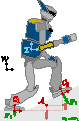
\includegraphics[width=0.5\columnwidth]{Uploaded/Images/framesAndAnchor.pdf} 
\vskip -0.5pc
\caption{Illustration of the anchor point position computation and of the reference frames used in Valinor. $\mathcal{W}$: world frame; $\mathcal{I}$: IMU frame; $\mathcal{C}_{i}$: frame of the $i$-th contact. For clarity, only the weighted average of the contact positions is shown. In this example, $\boldsymbol{F}_{2} = 2\boldsymbol{F}_{1}$ and so $\lambda_{2} = \frac{2}{3}$.}\label{fig:framesAndAnchor}
\end{center}
\vskip -1.5pc
\end{figure}

Based on this definition, we give the position and linear velocity of the anchor point in the IMU's frame, and its position in the world frame:
\begin{align} 
&{^{\mathcal{I}}}\boldsymbol{p}_{\mathcal{A}} = \sum^{n_{c}}_{i} \lambda_{i}  {^{\mathcal{I}}} \boldsymbol{p}_{{\mathcal{C}}_{i}}, \label{eq:imuAnchorPos} \\
&{^{\mathcal{I}}} \dot{\boldsymbol{p}}_{\mathcal{A}^{\prime}} = \sum^{n_{c}}_{i} \lambda_{i}  {^{\mathcal{I}}} \dot{\boldsymbol{p}}_{{\mathcal{C}}_{i}}, \label{eq:imuAnchorVel} \\
&\boldsymbol{p}_{\mathcal{A}} = \sum^{n_{c}}_{i} \lambda_{i} \boldsymbol{p}^{\star}_{{\mathcal{C}}_{i}}, \label{eq:anchorPointPos}
\end{align} 
with ${^{\mathcal{I}}} \boldsymbol{p}_{{\mathcal{C}}_{i}}$ the position and ${^{\mathcal{I}}} \dot{\boldsymbol{p}}_{{\mathcal{C}}_{i}}$ the linear velocity of the $i$-th contact in the IMU's frame, which are directly provided by the robot's joint encoders. $\boldsymbol{p}^{\star}_{{\mathcal{C}}_{i}}$ is the constant reference position of the $i$-th contact, which was its position at the instant it was created.
\textcolor{red}{What about p star and R star for the reference pose of the contacts? So we make clear they are different. But when should I talk about the reference pose of contacts? before or after ? Right above i talk about the fixed contact assumption.}
\textcolor{red}{Remove $\mathcal{A}^\prime$?}


\textcolor{red}{TODO}

\section{Tilt Observer with proof of convergence}
The proposed estimator relies on a highly accurate estimate of the IMU's tilt provided by a complementary filter, introduced in a previous work \textcolor{red}{citer}, which we will call \emph{Tilt Observer}. 

\subsection{Definition of the State Variables}
The Tilt Observer is able to provide estimates of the following two variables: 
\begin{itemize}
    \item $\boldsymbol{v}_{\mathcal{I}, l} \triangleq \boldsymbol{R}^{T}_{\mathcal{I}} \boldsymbol{v}_{\mathcal{I}} $ the linear velocity of the IMU's frame in the world frame, expressed in the frame of the IMU.
    \item $\boldsymbol{R}^{T}_{\mathcal{I}} \boldsymbol{e}_z$ the tilt of the IMU.
\end{itemize}
We thus define the state variables: 
\begin{alignat}{2}
&\boldsymbol{x}_{1} \triangleq \boldsymbol{v}_{\mathcal{I}, l} \quad &&, \boldsymbol{x}_{1} \in \mathbb{R}^{3}, \label{eq:x1} \\
&\boldsymbol{x}_{2} \triangleq \boldsymbol{R}^{T}_{\mathcal{I}} \boldsymbol{e}_z \quad &&, \boldsymbol{x}_{2} \in \mathbb{S}^{2}. \label{eq:x2}
\end{alignat} 
The set $\mathbb{S}^{2} \subset \mathbb{R}^{3}$ is the unit sphere centered at the origin, and defined as
\begin{equation}
    \mathbb{S}^{2} = \left\{ \boldsymbol{x} \in \mathbb{R}^{3} \vert \lVert \boldsymbol{x} \rVert=1 \right\}
\end{equation}

\begin{figure}[!t]
\begin{center}
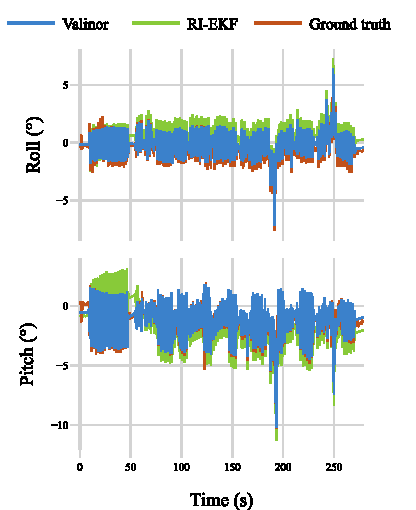
\includegraphics[width=0.5\columnwidth]{Uploaded/Images/tilt.pdf} 
\vskip -0.5pc
\caption{Tilt}\label{fig:tilt}
\end{center}
\vskip -1.5pc
\end{figure}

\textcolor{red}{This figure is uncited}

\subsection{Definition of the Measurements}
The measurements required by the Tilt Observer are:
\begin{itemize}
    \item $\boldsymbol{y}_{g}$ the signal of the IMU's gyrometer.
    \item $\boldsymbol{y}_{a}$ the signal of the IMU's accelerometer.
    \item $\boldsymbol{y}_{v}$ a measurement of $\boldsymbol{v}_{\mathcal{I}, l}$.
\end{itemize}
Since no sensor provides a direct measurement of $\boldsymbol{v}_{\mathcal{I}, l}$, we obtain $\boldsymbol{y}_{v}$ from an intermediate zero-velocity pseudo-measurement of the anchor point $\mathcal{A}$ in the world, giving:
\begin{equation}
    \boldsymbol{y}_v = - \left[\boldsymbol{y}_{g}\right]_{\times} {^{\mathcal{I}}}\boldsymbol{p}_{\mathcal{A}} - {^{\mathcal{I}}} \dot{\boldsymbol{p}}_{\mathcal{A}} \label{eq:yv}
\end{equation}
${^{\mathcal{I}}}\boldsymbol{p}_{\mathcal{A}}$ and ${^{\mathcal{I}}} \dot{\boldsymbol{p}}_{\mathcal{A}}$ are the position and linear velocity of the anchor point in the IMU's frame, obtained using\eqref{eq:imuAnchorPos} and \eqref{eq:imuAnchorVel}.

\subsection{Definition of the Filter}
As explained in \textcolor{red}{Cite}, the state dynamics of our system can be written:
\begin{align} 
&\dot{\boldsymbol{x}}_{1} = -\left[\boldsymbol{y}_{g}\right]_{\times} \boldsymbol{x}_{1} - g_{0}\boldsymbol{x}_{2} + \boldsymbol{y}_{a} , \label{eq:x1_dot} \\
&\dot{\boldsymbol{x}}_{2} = -\left[\boldsymbol{y}_{g}\right]_{\times} \boldsymbol{x}_{2}. \label{eq:x2_dot}
\end{align} 
We can then write a complementary filter which uses the system's dynamics as a feed-forward, and corrects the estimated state using the velocity measurement $\boldsymbol{y}_{v}$:
\begin{align} 
& \dot{\hat{\boldsymbol{x}}}_{1}  = - \left[\boldsymbol{y}_{g}\right]_{\times}\hat{\boldsymbol{x}}_{1} - g_{0} \hat{\boldsymbol{x}}_{2}^{\prime} + \boldsymbol{y}_{a} + \alpha_{1} \left(\boldsymbol{y}_{v} - \hat{\boldsymbol{x}}_{1}\right), \label{x1_dot} \\
    & \dot{\hat{\boldsymbol{x}}}_{2}^{\prime} = - \left[\boldsymbol{y}_{g}\right]_{\times} \hat{\boldsymbol{x}}_{2} - \frac{\alpha_{2}}{g_{0}} \left(\boldsymbol{y}_{v} - \hat{\boldsymbol{x}}_{1}\right), \\
    & \dot{\hat{\boldsymbol{x}}}_{2} = - \left[\boldsymbol{y}_{g} - \gamma \left[\hat{\boldsymbol{x}}_{2}\right]_{\times}\hat{\boldsymbol{x}}_{2}^{\prime}\right]_{\times} \hat{\boldsymbol{x}}_{2}.
\end{align} 
$\alpha_1$, $\alpha_2$ and $\gamma$ are positive scalar gains. $\hat{\boldsymbol{x}}_{1} $ and $\hat{\boldsymbol{x}}_{2} $ are estimates of $\boldsymbol{x}_{1} $ and $\boldsymbol{x}_{2} $, respectively. 

The particularity of the Tilt Observer, in comparison to similar complementary filters (e.g. \textcolor{red}{Martin2016}), is the use of an intermediate estimate of the tilt, denoted $\hat{\boldsymbol{x}}_{2}^{\prime}$. This intermediate variable allows for a fast convergence of $\hat{\boldsymbol{x}}_{2}$, while making sure it remains on the unit sphere. 


% \begin{alignat}{2}
%          &\boldsymbol{y}_{g}    && \triangleq \boldsymbol{\omega}_{\mathcal{I}, l}, \\
%          &\boldsymbol{y}_{a}    && \triangleq \boldsymbol{R}^{T}_{\mathcal{I}} \boldsymbol{a}_{\mathcal{I}} = \text{S}\! \left( \boldsymbol{\omega}_{\mathcal{I}, l} \right) \boldsymbol{v}_{\mathcal{I}, l} + \dot{\boldsymbol{v}}_{\mathcal{I}, l} + g_0 \boldsymbol{R}^{T}_{\mathcal{I}} \boldsymbol{e}_z, \\
%          &\boldsymbol{y}_{v}    && \triangleq \boldsymbol{v}_{\mathcal{I}, l},
% \end{alignat}

\subsection{Advantages of the Tilt Observer}
The use of a complementary filter for the Tilt Observer presents notable strengths in comparison to other methods like the commonly used Kalman Filter. First, it allows us to work in the frequency domain. This is particularily suitable for our model since the assumption of fixed contacts used to obtain the velocity measurement $\boldsymbol{y}_v$ is more valid in low frequency than in high frequency. In~\eqref{eq:x1_dot}, we thus use the IMU measurements for the high frequency variation of $\hat{\boldsymbol{x}}_{1}$, and $\boldsymbol{y}_v$ for its low frequency variation. Second, one iteration of the filter only consists in computing three equations, and is thus extremely computationally cheap, as will be shown in \textcolor{red}{Section}. Finally, the formulation as a complementary filter allows to conduct a convergence analysis of the estimation error, providing strong mathematical guarantees on the estimator's performances. Especially here, it has been shown in \textcolor{red}{Cite} that:
\begin{itemize}
    \item The dynamics of the estimation error is autonomous, and thus does not depend on the state. 
    \item The intermediate estimator $\left\{\hat{\boldsymbol{x}}_{1}, \hat{\boldsymbol{x}}_{2}^{\prime} \right\}$ is \emph{globally exponentially stable}, with respect to the origin $\left(0,0\right)$.
    \item The full estimator is \emph{almost globally asymptotically stable}, and locally \emph{exponentially stable}.
\end{itemize}

\section{Leg Odometry}

While the tilt of the IMU's frame in the world frame is estimated by the Tilt Observer, its position and yaw are obtained using Leg odometry. Once a contact $i$ is created, its pose is obtained by forward kinematics from the current IMU's frame pose and the robot's joint encoders. This initial pose, which we call the contact's reference pose $\left\{ \boldsymbol{p}^{\star}_{\mathcal{C}_{i}}, \boldsymbol{R}^{\star}_{\mathcal{C}_{i}}\right\}$, is then considered constant, allowing to recover the pose of the IMU's frame in the world frame. 
With the proposed pipeline, we thus leverage both the accuracy and mathematical guarantees provided by the Tilt Observer, and the robustness to drift provided by the Leg odometry. Similarly to the computation of the anchor point in Section~\ref{sec:anchor_point}, the contribution of contacts to the Leg odometry is weighted to trust more contacts which are the least prone to slippage.


\textcolor{red}{What about using the force ratio even for the correction of contacts?}
\subsection{Averaging of orientations and merging with tilt}

To obtain the yaw from contact information, we compute the weighted average between the reference orientation of the two most reliable contacts. In our case, we assume they are the contacts with the highest measured reaction force, as explained in Section~\ref{sec:anchor_point}. For each contact $i$, we can write:
\begin{equation}
    \boldsymbol{R}_{\mathcal{I}, i} = \boldsymbol{R}^{\star}_{\mathcal{C}_{i}} {}^{\mathcal{C}_{i}} \boldsymbol{R}_{\mathcal{I}} 
\end{equation}
We then compute the average $\boldsymbol{R}_{\mathcal{I}, \text{avg}}$ between both contacts using the formalism defined by SO(3) the Lie group of rotation matrices:
\begin{align}
    &\tilde{\boldsymbol{R}} = \boldsymbol{R}^{T}_{\mathcal{I}, 1} \boldsymbol{R}_{\mathcal{I}, 2}  \\
 & \boldsymbol{R}_{\mathcal{I}, \text{avg}} = \boldsymbol{R}_{\mathcal{I}, 1} \text{exp} \left( \lambda_{2} \text{vec}\left(\text{log} \left( \tilde{\boldsymbol{R}}\right)\right)  \right).
\end{align}
exp and log are the \emph{exponential} and \emph{logarithm} maps of SO(3). We note that for small angles, we can use the approximation:
\begin{equation}
log\left(\tilde{\boldsymbol{R}}\right) = \frac{1}{2} \left(\tilde{\boldsymbol{R}}-\tilde{\boldsymbol{R}}^{T}\right), \label{eq:log_small}
\end{equation}
Once the average orientation has been computed, we 


\textcolor{red}{Check if Log or log.}
\textcolor{red}{In the implementation, i don't do $R-R^T$}

%         stateObservation::Matrix3 diffRot = R1.transpose() * R2;

%         stateObservation::Vector3 diffRotVector =
%             (1.0 - u)
%             * stateObservation::kine::skewSymmetricToRotationVector(
%                 diffRot); // we perform the multiplication by the weighting coefficient now so a
%                           // zero coefficient gives a unit rotation matrix and not a zero matrix

%         stateObservation::AngleAxis diffRotAngleAxis = stateObservation::kine::rotationVectorToAngleAxis(diffRotVector);

%         stateObservation::Matrix3 diffRotMatrix =
%             stateObservation::kine::Orientation(diffRotAngleAxis).toMatrix3(); // exp( (1 - u) * log(R1^T R2) )
            
\subsection{Averaging of positions}
We use the updated orientation.
\begin{equation}
    \boldsymbol{p}_{\mathcal{I}} = \boldsymbol{p}_{\mathcal{A}} - \boldsymbol{R}_{\mathcal{I}} {}^{\mathcal{I}}\boldsymbol{p}_{\mathcal{A}} 
\end{equation}

\section{Experimental evaluation}

The proposed estimator has been evaluated accross two experimental scenarios on two different humanoid robots\footnote{we used the dataset built to evaluate the Kinetics Observer in \textcolor{red}{cite}}:
\begin{itemize}
    \item a walk on a flat ground over about 18 meters with the robot RHP Friends. This experiment was repeated 5 times, for a total distance of about 90 meters. 
    \item a multi-contact motion over about 2 meters with the robot HRP-5P. This motion involved an additional contact at the robot's left hand, and contacts on tilted obstacles. This experiments was repeated 4 times for a total distance of about 8 meters.
\end{itemize}

We compare Valinor, our proposed estimator, with the Right-Invariant EKF (RI-EKF) by \textcolor{red}{Hartley2020RIEKF}. For a fair comparison, both estimators received the same contact state information, obtained from a Schmitt Trigger applied to force sensor data (with thresholds set to 10\% and 15\% of the robot's weight).
Ground truth pose is obtained from a motion capture system (OptiTrack, 16 Prime\textsuperscript{X} 13 cameras), and ground truth velocity is computed via finite differences and filtered with a zero-phase low-pass filter.

The odometry performance of Valinor and the RI-EKF is evaluated against the ground truth trajectory using the Absolute Trajectory Error (ATE) and Relative Error (RE), as defined in \textcolor{red}{Zhang2018QuantitativeTrajectoryEvaluation}. ATE is computed after realigning the estimated trajectory to the ground truth, in order to minimize the squared error between them. The mean ATE allows to quantify the global consistency and fidelity of the estimated trajectory to the actual one, completed by its standard deviation which highlights the presence of large deviations. RE evaluates the estimation drift over segments of fixed distances. It is particularly relevant for proprioceptive odometry, as it is not affected by global drift, which is unavoidable without exteroceptive sensors. RE therefore provides valuable and easily interpretable insight into the expected local accuracy of the estimator over a given distance.

We compute separately the ATE and RE for lateral ($\boldsymbol{x}, \boldsymbol{y}$) and vertical ($\boldsymbol{z}$) translations, since these components are generally influenced by different factors. Accuracy in lateral translation would mainly rely on that of local displacements and yaw estimation, whereas accuracy in vertical translations would be affected by the accuracy of the estimation of the vertical local displacement, of the tilt, and the reliability of the contact height initialization. Similarily, angular errors in tilt and yaw are also evaluated independently.

Finally, we also assess the estimation of the IMU's linear velocity in the world. This velocity is expressed in the frame of the IMU such that it is not affected by errors in the orientation estimate. The velocity error is also separated into lateral and vertical components.

\subsection{Multi-contact}

We evaluated the performances of Valinor over a multi-contact motion, implying 

\begin{table*}[!b] 
\vskip -0.75pc
\setlength{\extrarowheight}{0.5ex}
\setlength{\tabcolsep}{1pt}
\caption{Mean and standard deviation (in parentheses) of errors computed during multi-contact motions. The 0.3 m Relative Error is represented. The best results for each metric are highlighted in bold.} \label{tab:multicontact-odometry-results}
\begin{center}
\vskip -1.25pc
{\footnotesize
    \begin{center}
        \begin{tabu}to\linewidth{| X[c] || X[c] | X[c] | X[c] | X[c] | X[c] | X[c] | X[c] | X[c] | X[c] | X[c] |}
            \hline
            \multirow{4}{*}{}          &       \multicolumn{4}{c|}{Translation [m]}         &    \multicolumn{4}{c|}{Orientation $[^{\circ}]$}  &    \multicolumn{2}{c|}{Linear velocity $[\text{m.s}^{-1}]$}     \\     
            \cline{2-11}
                        &    \multicolumn{2}{c|}{Lateral}    &     \multicolumn{2}{c|}{Vertical}      &     \multicolumn{2}{c|}{Tilt}    &    \multicolumn{2}{c|}{Yaw}    &   Lateral  &  Vertical \\ 
                        &    \multicolumn{2}{c|}{ \{$\boldsymbol{x}, \boldsymbol{y}$\}}    &     \multicolumn{2}{c|}{$\boldsymbol{z}$}      &     \multicolumn{2}{c|}{}    &    \multicolumn{2}{c|}{}    &   \{$\boldsymbol{x}, \boldsymbol{y}$\}  &  $\boldsymbol{z}$ \\
            \cline{2-11}
                        &    $\text{ATE}_{\left\{\boldsymbol{x}, \boldsymbol{y}\right\}}$  &    $\text{RE}_{\left\{\boldsymbol{x}, \boldsymbol{y}\right\}}$   &    $\text{ATE}_{\boldsymbol{z}}$      &     $\text{RE}_{\boldsymbol{z}}$   &    $\text{ATE}_{\left\{\text{r, p}\right\}}$  & $\text{RE}_{\left\{\text{r, p}\right\}}$ &  $\text{ATE}_{\text{yaw}}$ &  $\text{RE}_{\text{yaw}}$  &   $\text{Vel}_{\left\{\boldsymbol{x}, \boldsymbol{y}\right\}}$  &  $\text{Vel}_{\boldsymbol{z}}$  \\
            \hline     
            
            Valinor       &  \textbf{\getErrorResult{Multicontact}{Tilt}{AbserrorHrpeMulticontactA}{Transxy}{Meanabs}}   &  \textbf{\getErrorResult{Multicontact}{Tilt}{Relerror}{Transxy}{Meanabs}}  &  \getErrorResult{Multicontact}{Tilt}{AbserrorHrpeMulticontactA}{Transz}{Meanabs}  &  \textbf{\getErrorResult{Multicontact}{Tilt}{Relerror}{Transz}{Meanabs}}   &  \textbf{\getErrorResult{Multicontact}{Tilt}{AbserrorHrpeMulticontactA}{Tilt}{Meanabs}}     &  \textbf{\getErrorResult{Multicontact}{Tilt}{Relerror}{Tilt}{Meanabs}}    &   \textbf{\getErrorResult{Multicontact}{Tilt}{AbserrorHrpeMulticontactA}{Yaw}{Meanabs}}    &    \textbf{\getErrorResult{Multicontact}{Tilt}{Relerror}{Yaw}{Meanabs}}     &  \getErrorResult{Multicontact}{Tilt}{Velerror}{EstimateXy}{Meanabs}    &   \textbf{\getErrorResult{Multicontact}{Tilt}{Velerror}{EstimateZ}{Meanabs}}  \\ 
            (Proposed) &   (\getErrorResult{Multicontact}{Tilt}{AbserrorHrpeMulticontactA}{Transxy}{Std})   &   (\textbf{\getErrorResult{Multicontact}{Tilt}{Relerror}{Transxy}{Std}})   &  (\getErrorResult{Multicontact}{Tilt}{AbserrorHrpeMulticontactA}{Transz}{Std})  &     (\textbf{\getErrorResult{Multicontact}{Tilt}{Relerror}{Transz}{Std}})    &       (\textbf{\getErrorResult{Multicontact}{Tilt}{AbserrorHrpeMulticontactA}{Tilt}{Std}})   &   (\textbf{\getErrorResult{Multicontact}{Tilt}{Relerror}{Tilt}{Std}})   &      (\textbf{\getErrorResult{Multicontact}{Tilt}{AbserrorHrpeMulticontactA}{Yaw}{Std}})  &    (\textbf{\getErrorResult{Multicontact}{Tilt}{Relerror}{Yaw}{Std}})   &  (\getErrorResult{Multicontact}{Tilt}{Velerror}{EstimateXy}{Std})   &   (\textbf{\getErrorResult{Multicontact}{Tilt}{Velerror}{EstimateZ}{Std}})  \\ 
            \hline 

            \multirow{2}{*}{RI-EKF \cite{1}}    &  \getErrorResult{Multicontact}{Hartley}{AbserrorHrpeMulticontactA}{Transxy}{Meanabs}   &  \getErrorResult{Multicontact}{Hartley}{Relerror}{Transxy}{Meanabs}  &  \textbf{\getErrorResult{Multicontact}{Hartley}{AbserrorHrpeMulticontactA}{Transz}{Meanabs}}  &  \getErrorResult{Multicontact}{Hartley}{Relerror}{Transz}{Meanabs}   &  \getErrorResult{Multicontact}{Hartley}{AbserrorHrpeMulticontactA}{Tilt}{Meanabs}     &  \getErrorResult{Multicontact}{Hartley}{Relerror}{Tilt}{Meanabs}    &   \getErrorResult{Multicontact}{Hartley}{AbserrorHrpeMulticontactA}{Yaw}{Meanabs}    &    \getErrorResult{Multicontact}{Hartley}{Relerror}{Yaw}{Meanabs}   &  \getErrorResult{Multicontact}{Hartley}{Velerror}{EstimateXy}{Meanabs}    &   \getErrorResult{Multicontact}{Hartley}{Velerror}{EstimateZ}{Meanabs}  \\ 
            &   (\getErrorResult{Multicontact}{Hartley}{AbserrorHrpeMulticontactA}{Transxy}{Std})   &   (\getErrorResult{Multicontact}{Hartley}{Relerror}{Transxy}{Std})   &  (\textbf{\getErrorResult{Multicontact}{Hartley}{AbserrorHrpeMulticontactA}{Transz}{Std}})  &     (\getErrorResult{Multicontact}{Hartley}{Relerror}{Transz}{Std})    &       (\getErrorResult{Multicontact}{Hartley}{AbserrorHrpeMulticontactA}{Tilt}{Std})   &   (\getErrorResult{Multicontact}{Hartley}{Relerror}{Tilt}{Std})   &      (\getErrorResult{Multicontact}{Hartley}{AbserrorHrpeMulticontactA}{Yaw}{Std})  &    (\getErrorResult{Multicontact}{Hartley}{Relerror}{Yaw}{Std})    &  (\getErrorResult{Multicontact}{Hartley}{Velerror}{EstimateXy}{Std})    &   (\getErrorResult{Multicontact}{Hartley}{Velerror}{EstimateZ}{Std})  \\ 
            \hline     
        \end{tabu}
    \end{center}
}
\end{center}
\vskip -0.25pc
\end{table*}





\subsection{Walk on flat floor}
Show table and plot of pose and vel. Focus on tilt.

\begin{figure}[!t]
\begin{center}
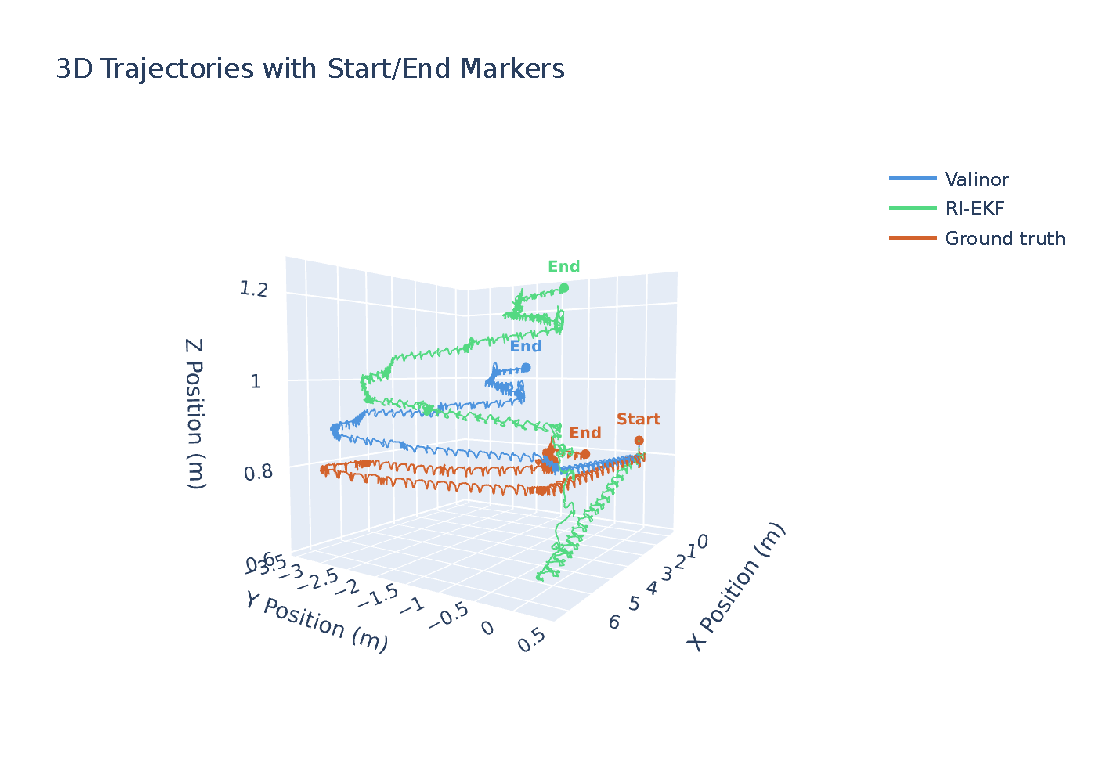
\includegraphics[width=\columnwidth]{Uploaded/Images/3d_traj.pdf} 
\vskip -0.5pc
\caption{Tilt}\label{fig:3d_traj}
\end{center}
\vskip -1.5pc
\end{figure}

We can see from Table~\ref{tab:flat-odometry-results} that the yaw estimation made by the RI-EKF is slightly better than that of Valinor. We explain this by the fact this orientation comes only from 


\begin{table*}[!b] 
\vskip -0.75pc
\setlength{\extrarowheight}{0.5ex}
\setlength{\tabcolsep}{1pt}
\caption{Mean and standard deviation (in parentheses) of errors computed during the flat odometry. The 1 m Relative Error is represented. The best results for each metric are highlighted in bold.} \label{tab:flat-odometry-results}
\begin{center}
\vskip -1.25pc
{\footnotesize
    \begin{center}
        \begin{tabu}to\linewidth{| X[c] || X[c] | X[c] | X[c] | X[c] | X[c] | X[c] | X[c] | X[c] | X[c] | X[c] |}
            \hline
            \multirow{4}{*}{}          &       \multicolumn{4}{c|}{Translation [m]}         &    \multicolumn{4}{c|}{Orientation $[^{\circ}]$}  &    \multicolumn{2}{c|}{Linear velocity $[\text{m.s}^{-1}]$}     \\     
            \cline{2-11}
                        &    \multicolumn{2}{c|}{Lateral}    &     \multicolumn{2}{c|}{Vertical}      &     \multicolumn{2}{c|}{Tilt}    &    \multicolumn{2}{c|}{Yaw}    &   Lateral  &  Vertical \\ 
                        &    \multicolumn{2}{c|}{ \{$\boldsymbol{x}, \boldsymbol{y}$\}}    &     \multicolumn{2}{c|}{$\boldsymbol{z}$}      &     \multicolumn{2}{c|}{}    &    \multicolumn{2}{c|}{}    &   \{$\boldsymbol{x}, \boldsymbol{y}$\}  &  $\boldsymbol{z}$ \\
            \cline{2-11}
                        &    $\text{ATE}_{\left\{\boldsymbol{x}, \boldsymbol{y}\right\}}$  &    $\text{RE}_{\left\{\boldsymbol{x}, \boldsymbol{y}\right\}}$   &    $\text{ATE}_{\boldsymbol{z}}$      &     $\text{RE}_{\boldsymbol{z}}$   &    $\text{ATE}_{\left\{\text{r, p}\right\}}$  & $\text{RE}_{\left\{\text{r, p}\right\}}$ &  $\text{ATE}_{\text{yaw}}$ &  $\text{RE}_{\text{yaw}}$  &   $\text{Vel}_{\left\{\boldsymbol{x}, \boldsymbol{y}\right\}}$  &  $\text{Vel}_{\boldsymbol{z}}$  \\
            \hline     
            
            Valinor       &  \getErrorResult{Flatodometry}{Tilt}{AbserrorKoTrobobdRhpsaA}{Transxy}{Meanabs}   &  \textbf{\getErrorResult{Flatodometry}{Tilt}{Relerror}{Transxy}{Meanabs}}  &  \textbf{\getErrorResult{Flatodometry}{Tilt}{AbserrorKoTrobobdRhpsaA}{Transz}{Meanabs}}  &  \textbf{\getErrorResult{Flatodometry}{Tilt}{Relerror}{Transz}{Meanabs}}   &  \textbf{\getErrorResult{Flatodometry}{Tilt}{AbserrorKoTrobobdRhpsaA}{Tilt}{Meanabs}}     &  \textbf{\getErrorResult{Flatodometry}{Tilt}{Relerror}{Tilt}{Meanabs}}    &   \textbf{\getErrorResult{Flatodometry}{Tilt}{AbserrorKoTrobobdRhpsaA}{Yaw}{Meanabs}}    &    \getErrorResult{Flatodometry}{Tilt}{Relerror}{Yaw}{Meanabs}     &  \getErrorResult{Flatodometry}{Tilt}{Velerror}{EstimateXy}{Meanabs}    &   \getErrorResult{Flatodometry}{Tilt}{Velerror}{EstimateZ}{Meanabs}  \\ 
            (Proposed) &   (\getErrorResult{Flatodometry}{Tilt}{AbserrorKoTrobobdRhpsaA}{Transxy}{Std})   &   (\textbf{\getErrorResult{Flatodometry}{Tilt}{Relerror}{Transxy}{Std}})   &  (\textbf{\getErrorResult{Flatodometry}{Tilt}{AbserrorKoTrobobdRhpsaA}{Transz}{Std}})  &     (\textbf{\getErrorResult{Flatodometry}{Tilt}{Relerror}{Transz}{Std}})    &       (\textbf{\getErrorResult{Flatodometry}{Tilt}{AbserrorKoTrobobdRhpsaA}{Tilt}{Std}})   &   (\textbf{\getErrorResult{Flatodometry}{Tilt}{Relerror}{Tilt}{Std}})   &      (\textbf{\getErrorResult{Flatodometry}{Tilt}{AbserrorKoTrobobdRhpsaA}{Yaw}{Std}})  &    (\getErrorResult{Flatodometry}{Tilt}{Relerror}{Yaw}{Std})   &  (\getErrorResult{Flatodometry}{Tilt}{Velerror}{EstimateXy}{Std})   &   (\getErrorResult{Flatodometry}{Tilt}{Velerror}{EstimateZ}{Std})  \\ 
            \hline 

            \multirow{2}{*}{RI-EKF \cite{1}}    &  \textbf{\getErrorResult{Flatodometry}{Hartley}{AbserrorKoTrobobdRhpsaA}{Transxy}{Meanabs}}   &  \getErrorResult{Flatodometry}{Hartley}{Relerror}{Transxy}{Meanabs}  &  \getErrorResult{Flatodometry}{Hartley}{AbserrorKoTrobobdRhpsaA}{Transz}{Meanabs}  &  \getErrorResult{Flatodometry}{Hartley}{Relerror}{Transz}{Meanabs}   &  \getErrorResult{Flatodometry}{Hartley}{AbserrorKoTrobobdRhpsaA}{Tilt}{Meanabs}     &  \getErrorResult{Flatodometry}{Hartley}{Relerror}{Tilt}{Meanabs}    &   \getErrorResult{Flatodometry}{Hartley}{AbserrorKoTrobobdRhpsaA}{Yaw}{Meanabs}    &    \textbf{\getErrorResult{Flatodometry}{Hartley}{Relerror}{Yaw}{Meanabs}}   &  \textbf{\getErrorResult{Flatodometry}{Hartley}{Velerror}{EstimateXy}{Meanabs}}    &   \getErrorResult{Flatodometry}{Hartley}{Velerror}{EstimateZ}{Meanabs}  \\ 
            &   (\textbf{\getErrorResult{Flatodometry}{Hartley}{AbserrorKoTrobobdRhpsaA}{Transxy}{Std}})   &   (\getErrorResult{Flatodometry}{Hartley}{Relerror}{Transxy}{Std})   &  (\getErrorResult{Flatodometry}{Hartley}{AbserrorKoTrobobdRhpsaA}{Transz}{Std})  &     (\getErrorResult{Flatodometry}{Hartley}{Relerror}{Transz}{Std})    &       (\getErrorResult{Flatodometry}{Hartley}{AbserrorKoTrobobdRhpsaA}{Tilt}{Std})   &   (\getErrorResult{Flatodometry}{Hartley}{Relerror}{Tilt}{Std})   &      (\getErrorResult{Flatodometry}{Hartley}{AbserrorKoTrobobdRhpsaA}{Yaw}{Std})  &    (\textbf{\getErrorResult{Flatodometry}{Hartley}{Relerror}{Yaw}{Std}})    &  (\textbf{\getErrorResult{Flatodometry}{Hartley}{Velerror}{EstimateXy}{Std}})    &   (\textbf{\getErrorResult{Flatodometry}{Hartley}{Velerror}{EstimateZ}{Std}})  \\ 
            \hline     
        \end{tabu}
    \end{center}
}
\end{center}
\vskip -0.25pc
\end{table*}





\subsection{Computation times comparison}


\subsection{References}

References should appear in a separate bibliography at the end of the paper, with items referred to by numerals in square brackets \cite{1,3,4,5}. Times New Roman 10 pt is used for references \cite{2}. References should be complete in the IJCAS style shown in the Reference section of this article. An article should include vol., no., pages, and year.



\section{CONCLUSION}

Opening: include a correction of the contact pose references.  Gyrometer and accelerometer biases.



\appendix

The author(s) can insert an appendix with a meaningful title here.



\section*{DECLARATIONS}

\subsection*{Conflict of Interest}
Always applicable and includes interests of a financial or personal nature. For example, ``The authors declare that there is no competing financial interest or personal relationship that could have appeared to influence the work reported in this paper.''

\subsection*{Authors' Contributions}
If there is one more author, please ensure that all authors' contributions are individually mentioned with their full names.

\subsection*{Funding }
It should be provided in the Declarations, separate from the Acknowledgements. If any of these declarations listed are not relevant to the content of your submission, please state that this declaration is ``Not Applicable''.




\begin{reference}
\bibitem{1} \doi{R. C. Baker and B. Charlie, ``Nonlinear unstable systems,'' \textit{International Journal of Control}, vol. 23, no. 4, pp. 123-145, 1989.}{10.1007s/s12555-xxx-xxxx-x}

\bibitem{2} G.-D. Hong, ``Linear controllable systems,'' \textit{Nature}, vol. 135, no. 5, pp. 18-27, 1990. 

\bibitem{3} K.-S. Hong and C. S. Kim, ``Linear stable systems,'' \textit{IEEE Transactions on Automatic Control}, vol. 33, no. 3, pp. 1234-1245, 1993. 

\bibitem{4} Z. Shiler, S. Filter, and S. Dubowski, ``Time optimal paths and acceleration lines of robotic manipulators,'' \textit{Proc. of the 26th Conference on Decision and Control}, pp. 98-99, 1987.

\bibitem{5}  M. Young, \textit{The Technical Writer's Handbook}, Mill Valley, Seoul, 1989.

\bibitem{6}  Y. Feng, H. Wang, H. Lu, C. Chang, L. Luo, and F. Yang, ``A novel faster all-pair shortest path algorithm based on the matrix multiplication for GPUs,'' \textit{arXiv preprint} arXiv:2208.04514, 2022.

\bibitem{7} ``Reinforcement learning,'' Wikipedia, [Online]. Available: \href{https://en.wikipedia.org/wiki/Reinforcement_learning}{https://en.wikipedia.org/wiki/Reinforcement\_learning}. [Accessed: March 24, 2025].
\end{reference}


% \biography{Uploaded/Arnaud.png}{Arnaud Demont}{received the M.S. degree in mechanical engineering with a specialization in mechatronics and systems from the National Institute of Applied Sciences of Lyon, France, and a second M.S. degree in automation and robotics in intelligent systems from the University of  Technology of Compiègne, France, in 2021 and 2023 respectively. He is currently pursuing the PhD degree of the Université Paris-Saclay, France, within the CRNS-AIST Joint Robotics Laboratory in Tsukuba, Japan. His research interests include state estimation for legged robots, multi-sensor fusion, and mobile robot perception and autonomous navigation.
% }

% \biography{Uploaded/Mehdi.png}{Mehdi Benallegue}{holds an engineering degree from the National Institute of Computer Science (INI) in Algeria, obtained in 2007. He earned a master's degree from the University of Paris 7, France, in 2008, and a Ph.D. from the University of Montpellier 2, France, in 2011. His research took him to the Franco-Japanese Robotics Laboratory in Tsukuba, Japan, and to INRIA Grenoble, France. He also worked as a postdoctoral researcher at the Collège de France and at LAAS CNRS in Toulouse, France. Currently, he is a Research Associate with CNRS AIST Joint robotics Laboratory in Tsukuba, Japan. His research interests include robot estimation and control, legged locomotion, biomechanics, neuroscience, and computational geometry.
% }

% \biography{Uploaded/Aziz.png}{Prof. Abdelaziz Benallegue}{received the B.S. degree in electronics engineering from Algiers National Polytechnic School, Algeria in 1986 and both the M.S. and Ph.D. degrees in automatic control and robotics from University of Pierre and Marie Curie, Paris 6 (currently Sorbonne University), France in 1987 and 1991 respectively. He was Associate professor in Automatic Control and Robotics at the University Pierre et Marie Curie, Paris 6 (currently Sorbonne University) from 1992 to 2002. In September 2002, he joined the University of Versailles St Quentin as full Professor assigned. He was a CNRS delegate at JRL-AIST, Japan for three years, between 2016 and 2022. His research activities are mainly related to linear and non-linear estimation and control theory (adaptive control, robust control, neural learning control, observers, multi-sensor fusion, etc.) with applications in robotics (humanoid robots, aerial robots, manipulator robots, etc.).
% }

\clearafterbiography
\relax 

\end{document}

